\chapter{ESTRATÉGIA DE INVERSÃO DO MODELO DE VELOCIDADES}
\label{cap9}

A estratégia de otimização do modelo de velocidades é baseada no método de empilhamento Elemento de Reflexão Comum (ERC), na NIP tomografia \cite{niptomo} e na Stereo tomografia \cite{stereo}.
O método ERC é uma alternativa ao empilhamento convencional no domínio do Ponto Médio Comum (PMC), tem como
objetivo a construção da seção empilhada a partir de um conjunto de seções de afastamento constante e
fornecer parâmetros importantes na construção do macro modelo de velocidades \cite{cre}.

Estes parâmetros são o raio de curvatura $R_{NIP}$ e o ângulo de emergência do raio normal $\beta_0$ dados para
uma frente de onda hipotética (Onda PIN) que se origina sobre o refletor em um ponto chamado de Ponto de Incidência Normal
(PIN) \cite{hubral}. Assim, a estratégia de inversão do modelo de velocidades consiste em, a partir dos parâmetros $R_{NIP}$ e $\beta_0$, encontrar o modelo de velocidades que localiza as fontes
pontuais PIN sobre os refletores em profundidade.

\begin{figure}[H]
\caption{Modelo de velocidades de três camadas com velocidades iguais a $1.508Km/s$,
$1.690Km/s$ e $2.000Km/s$, respectivamente. Este modelo é utilizado para a obtenção da seção
empilhada ERC através do empilhamento ERC.}
\begin{center}
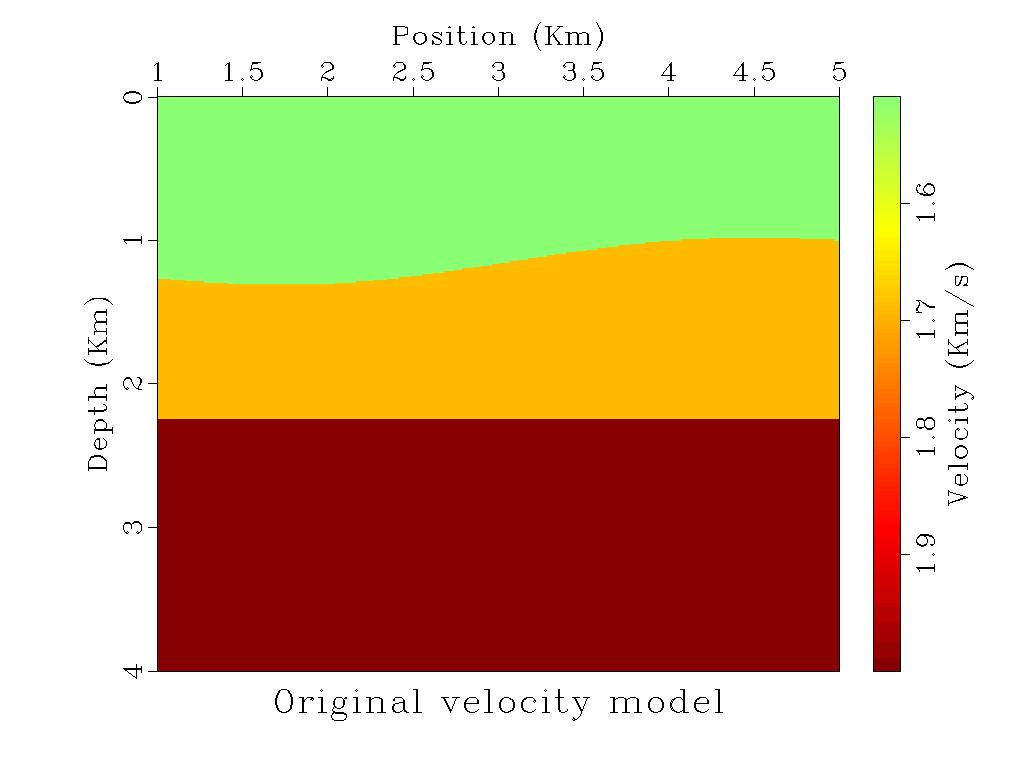
\includegraphics[scale=0.3]{images/mod1.jpeg}
\vspace{-0.3cm}
\end{center}
\begin{center}
 Fonte: Do Autor.
\end{center}
\label{fig:9.1}
\end{figure}

\begin{figure}[H]
\caption{Modelo de velocidades de três camadas com velocidades iguais a $1.508Km/s$,
$1.690Km/s$ e $2.000Km/s$, respectivamente. Este modelo é utilizado para a obtenção da seção
empilhada ERC através do empilhamento ERC.}
\begin{center}
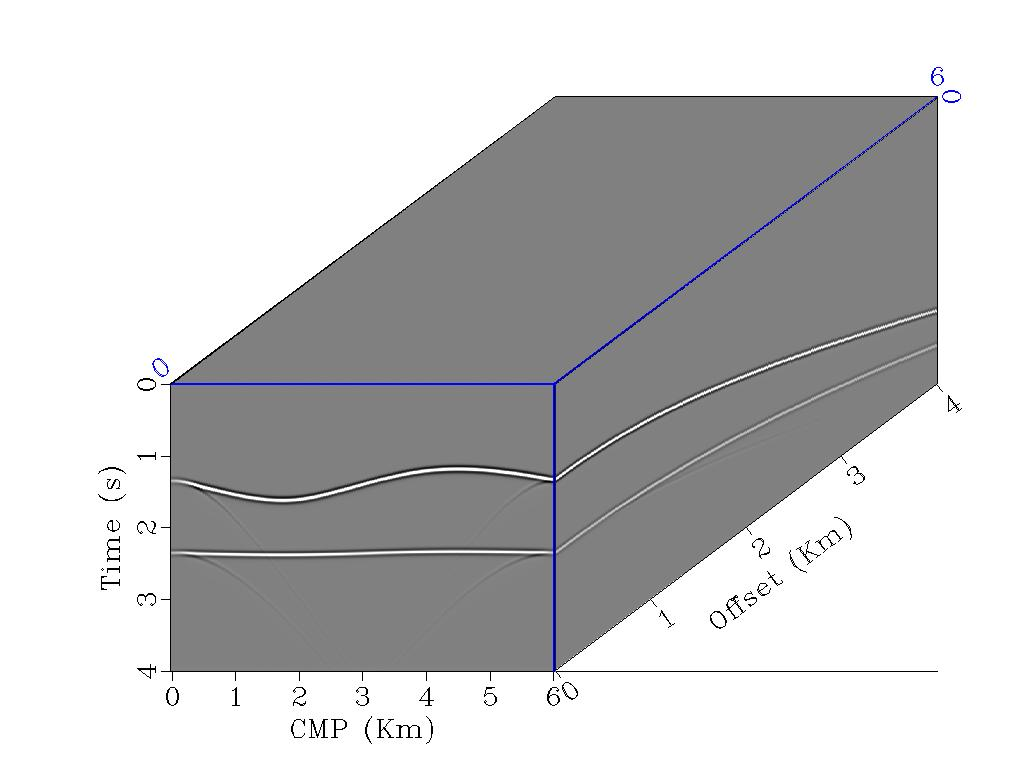
\includegraphics[scale=0.3]{images/datacube.jpeg}
\vspace{-0.3cm}
\end{center}
\begin{center}
 Fonte: Do Autor.
\end{center}
\label{fig:9.2}
\end{figure}

O nosso algoritmo para a inversão do modelo de velocidades em profundidade inicia com a obtenção dos dados
pré empilhados no domínio do PMC $m$ e do meio afastamento $h$ na Figura \ref{fig:9.2}. Estes dados foram
produzidos partir da modelagem Kirchhoff do modelo de velocidades
da Figura \ref{fig:9.1}. Este modelo possui três camadas com velocidades iguais a $1.508Km/s$,
$1.690Km/s$ e $2.000Km/s$, respectivamente. A modelagem Kirchhoff é feita através dos programas
de modelagem disponíveis no pacote de processamento sísmico Madagascar \cite{madagascar},
os mesmos utilizados no experimento numérico do Capítulo 6 para o refletor Gaussiano.

Em seguida, a partir dos dados sísmicos modelados, realizamos a otimização dos parâmetros $R_{NIP}$
e $\beta_0$ através do Very Fast Simulated Annealing (VFSA) e da utilização da aproximação de tempo
de trânsito do SRC não hiperbólico, com a metodologia descrita no Capítulo 4.
Estes parâmetros permitem a obtenção
das curvas de tempo de trânsito ERC para a realização do empilhamento das amplitudes. 
A próxima etapa consiste em estabelecer as famílias ERC onde são definidas as
curvas de tempo de trânsito ERC .

Assim, utilizamos a metodologia de interpolação com filtros FPE, descrita no Capítulo 4 e utilizada
no experimento numérico do Capítulo 7, para aumentar o número de amostras
dos dados modelados
no domínio do PMC, de modo a possibilitar amostragem suficiente para a
obtenção das famílias ERC e a subsequente obtenção da
seção de afastamento nulo através do empilhamento ERC. O empilhamento ERC
é realizado através da medida da coerência (semblance) das amplitudes sobre as curvas de tempo de trânsito
ERC em uma família ERC de traços sísmicos. As amplitudes são empilhadas sobre esta curva e atribuídas
às coordenadas ($m_0$,$t_0$) na seção empilhada ERC.
O algoritmo para a obtenção da seção empilhada ERC é apresentado no fluxograma a seguir.

\begin{figure}[H]
\caption{Representação esquemática do algoritmo para a obtenção da seção empilhada ERC
através do empilhamento ERC. Dados de entrada e saída de cada etapa do algoritmo.}
\begin{center}
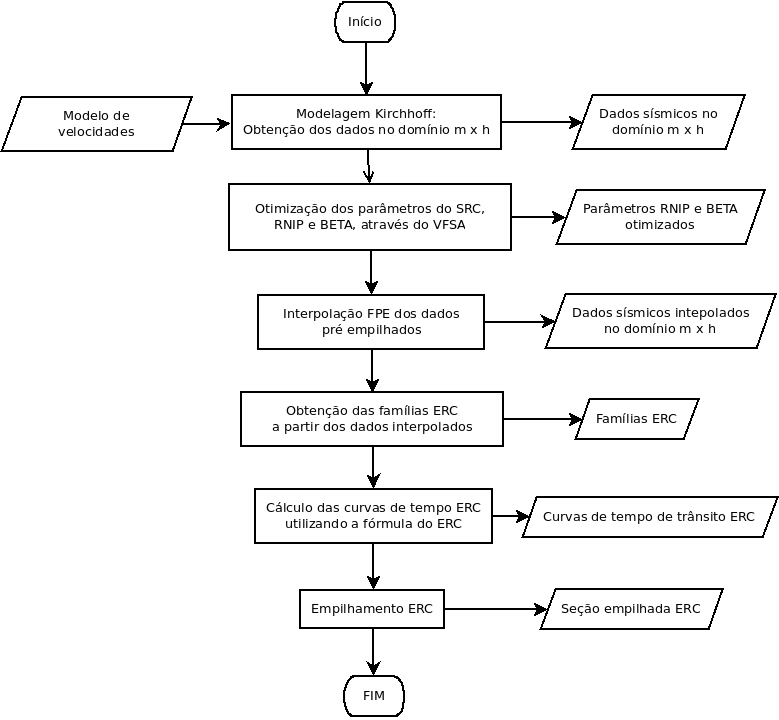
\includegraphics[scale=0.5]{images/fluxoemperc.png}
\vspace{-0.3cm}
\end{center}
\begin{center}
 Fonte: Do Autor.
\end{center}
\label{alg:9.1}
\end{figure}

\begin{figure}[H]
\caption{Seção empilhada ERC obtida através do empilhamento ERC
do modelo de velocidades da Figura \ref{fig:9.1}.}
\begin{center}
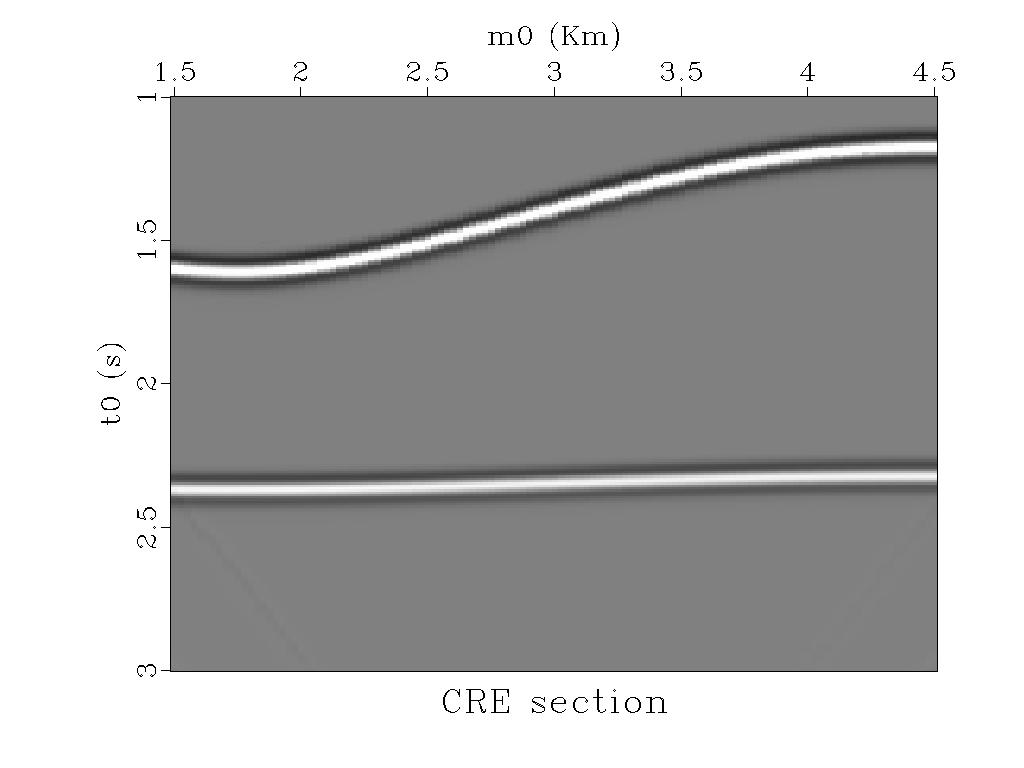
\includegraphics[scale=0.3]{images/stacked.jpeg}
\vspace{-0.3cm}
\end{center}
\begin{center}
 Fonte: Do Autor.
\end{center}
\label{fig:9.3}
\end{figure}

Após a obtenção da seção empilhada ERC através do empilhamento ERC dos dados sísmicos de reflexão
obtidos da modelagem Kirchhoff do modelo de velocidades da Figura \ref{fig:9.1},
com três camadas com as velocidades $1.508Km/s$, $1.690Km/s$ e $2.000Km/s$ respectivamente,
utilizando a metodologia de empilhamento ERC descrita no Capítulo 8,
realizamos o picking interativo dos tempos de trânsito, selecionando manualmente alguns
pontos sobre os refletores na seção empilhada ERC
(Ver Figura \ref{fig:9.4}, pontos em amarelo).
Estes tempos de trânsito selecionados na seção de afastamento nulo (seção empilhada ERC)
são os tempos duplos $t_0$ dos raios normais que partem da coordenada $m_0$
de um PMC na superfície de aquisição e incidem normais ao refletor no ponto PIN (Figura \ref{fig:9.5}).

Os tempos de trânsito $t_0$ escolhidos são utilizados para traçar raios normais
a partir da superfície de aquisição em direção ao modelo de velocidades
em profundidade,
de modo a determinar a possível localização do refletor no modelo
para um determinado modelo de velocidades.
O traçamento continua até que metade do tempo de trânsito $t_0$ seja consumido.
O modelo de velocidades inicial é um modelo de velocidade constante igual à velocidade $v_0$
próxima da superfície de aquisição.

\begin{figure}[H]
\caption{Picking manual dos tempos de trânsito sobre um refletor da seção empilhada ERC. Os pontos
em amarelo são os pares $t_0$ e $m_0$ escolhidos.}
\begin{center}
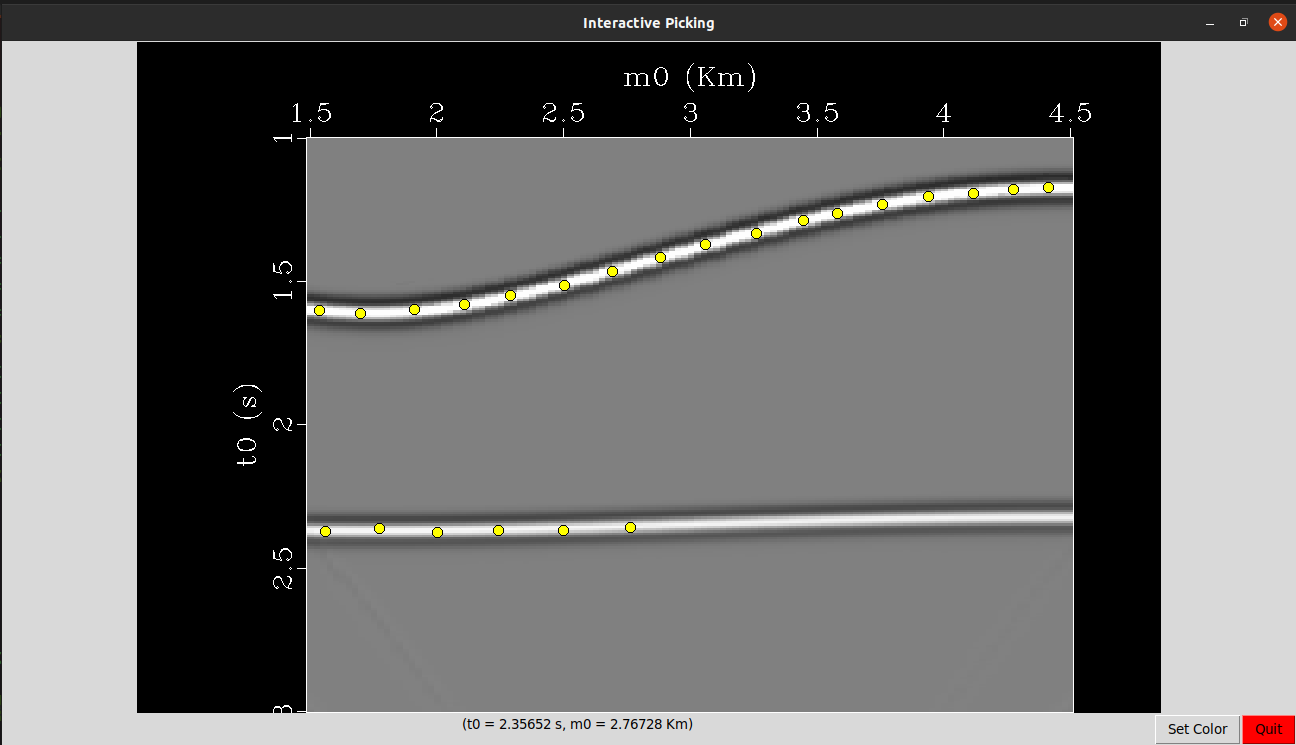
\includegraphics[scale=0.3]{images/picking.png}
\vspace{-0.3cm}
\end{center}
\begin{center}
 Fonte: Do Autor.
\end{center}
\label{fig:9.4}
\end{figure}

\begin{figure}[H]
\caption{Exemplo esquemático do traçamento de raios normais a partir de uma coordenada de um CMP $m_0$
na superfície de aquisição em direção ao modelo em profundidade.
O raio normal (seta) parte da superfície de aquisição com ângulo $\beta_0$ e incide normal
ao refletor no Ponto de Incidência Normal (PIN).}
\begin{center}
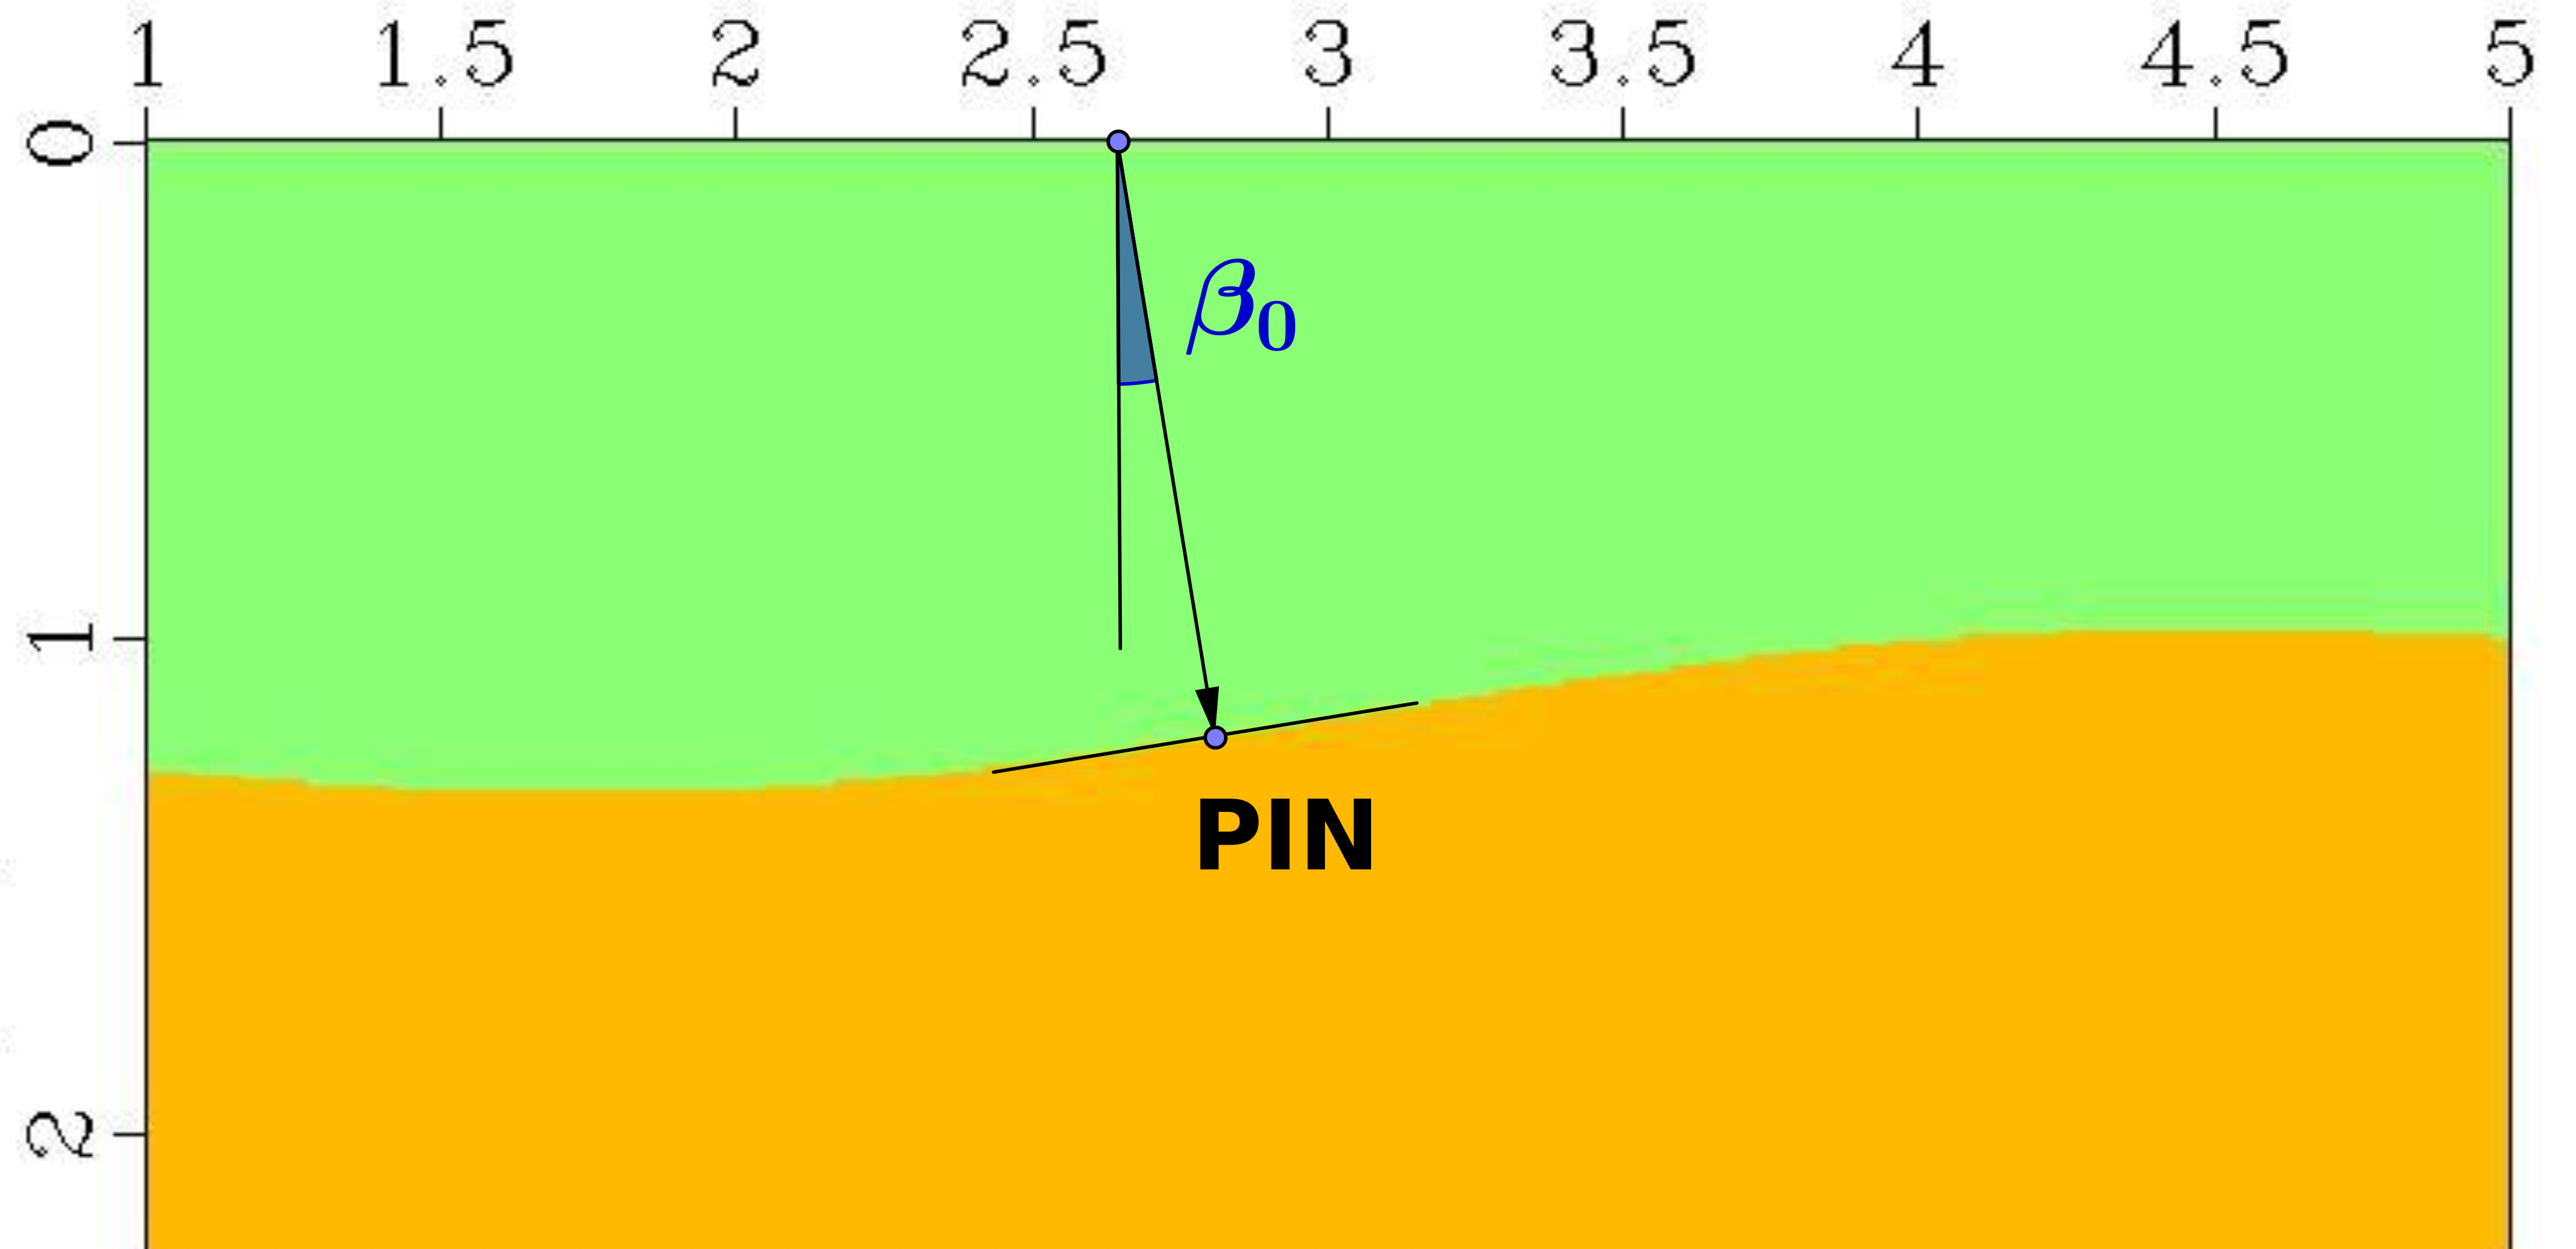
\includegraphics[scale=0.5]{images/modelagem.png}
\vspace{-0.3cm}
\end{center}
\begin{center}
 Fonte: Do Autor.
\end{center}
\label{fig:9.5}
\end{figure}

\begin{figure}[H]
\caption{Exemplo de traçamento do raio utilizando o programa \textit{sfrays2}
em direção a um modelo de velocidades suavizado.
Este programa está disponível no pacote de processamento sísmico Madagascar e foi
modificado para obter a localização das fontes PIN nos modelos de velocidade deste relatório.}
\begin{center}
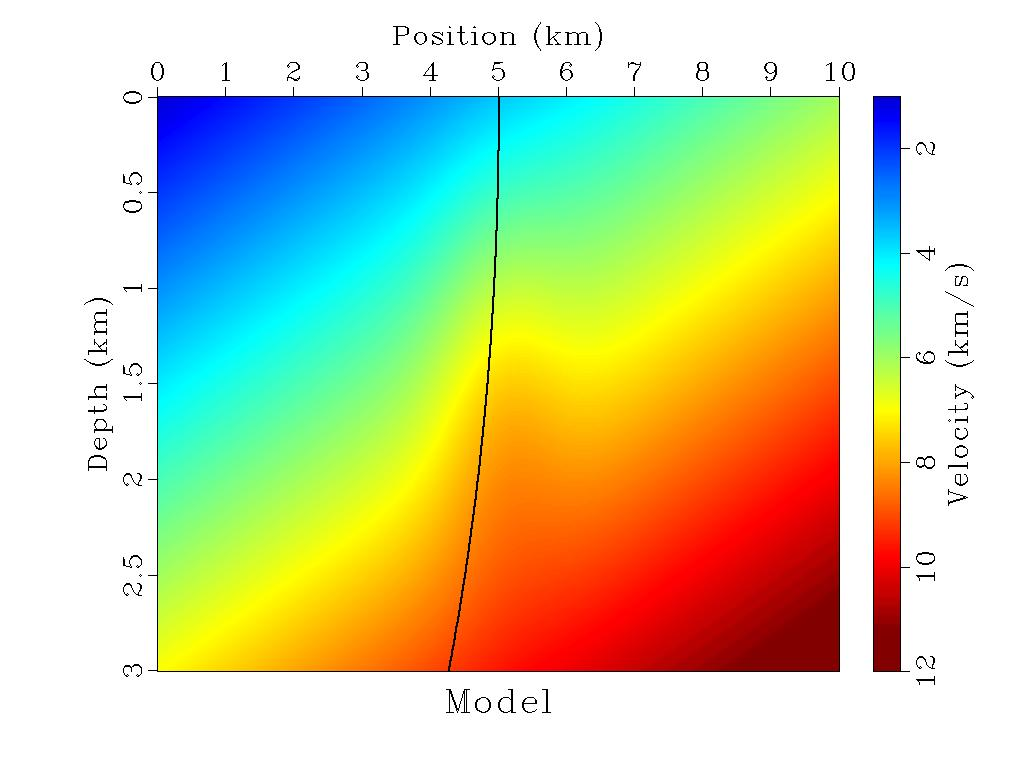
\includegraphics[scale=0.3]{images/raiomodelo.jpg}
\vspace{-0.3cm}
\end{center}
\begin{center}
 Fonte: Do Autor.
\end{center}
\label{fig:9.6}
\end{figure}

\begin{figure}[H]
\caption{Exemplo de traçamento do raio utilizando o programa \textit{sfrays2}
de um ponto no modelo de velocidades suavizado em direção à superfície de aquisição.
Este programa está disponível no pacote de processamento sísmico Madagascar e foi
modificado para a realização da modelagem direta neste relatório.}
\begin{center}
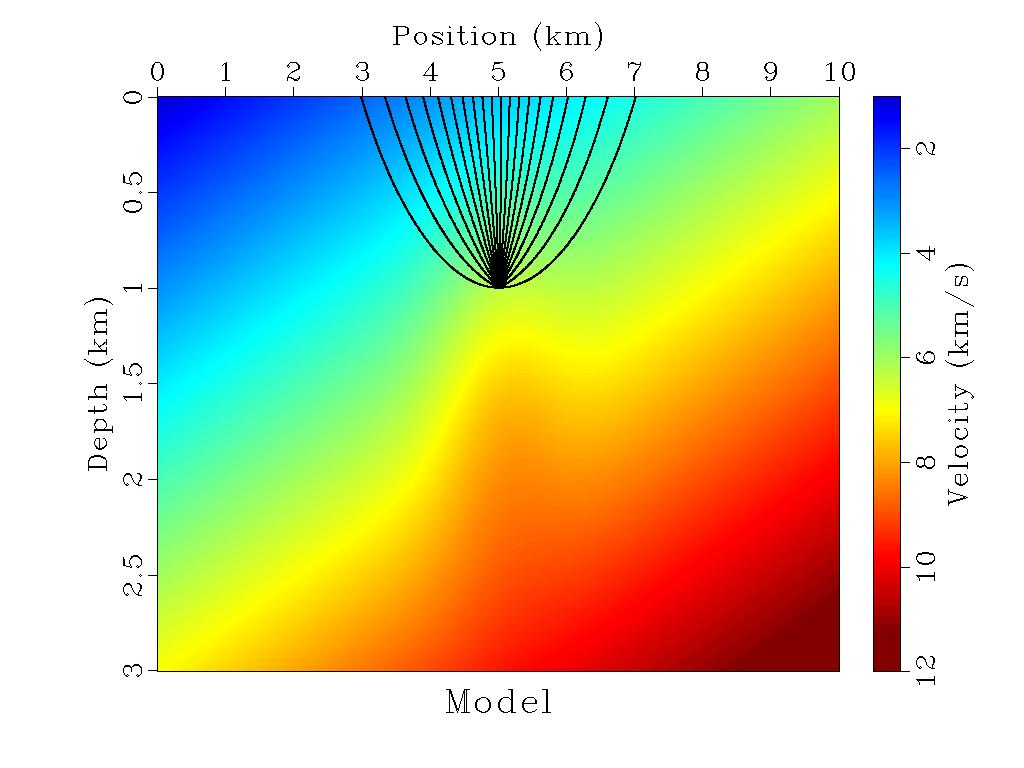
\includegraphics[scale=0.3]{images/raioleque.jpg}
\vspace{-0.3cm}
\end{center}
\begin{center}
 Fonte: Do Autor.
\end{center}
\label{fig:9.7}
\end{figure}

O programa para o traçamento de raios foi desenvolvido
utilizando as interfaces da Application Programming Interface (API)
do pacote de processamento sísmico Madagascar\footnote{Este pacote de processamento sísmico
está disponíveil no site oficial do pacote Madagascar em \url{http://www.ahay.org/wiki/Main_Page}. 
Os programas do pacote e a interface de traçamento de raios é disponibilizada sob
os termos da licensa de uso GPL-3.0 para software livre disponível
em \url{https://www.gnu.org/licenses/gpl-3.0.txt}.} \cite{madagascar}
e da construção de uma versão modificada do programa para traçamento de raios 
\textit{sfrays2} que realiza o traçamento cinemático dos raios
através do método Runge-Kutta. Estes raios podem ser traçados da superfície de aquisição em
direção ao modelo de velocidades em profundidade (Figura \ref{fig:9.6}) e de um
ponto no modelo de velocidades em direção à superfície de aquisição (Figura \ref{fig:9.7}).
O programa também permite obter as coordenadas de chegada dos raios e o tempo de trânsito.

Cada raio normal é iniciado na superfície de aquisição na posição da coordenada $m_0$ e lançado no modelo 
com a direção inicial dada pelo parâmetro $\beta_0$ (Figura \ref{fig:9.5}).
O ponto final do raio é a possível localização do refletor em profundidade
e onde será estabelecida a localização das fontes pontuais PIN para o modelo de velocidades.
O vetor vagarosidade neste ponto é
normal ao refletor, e com estas informações, o modelo de velocidades inicial é configurado \cite{niptomo}.

\begin{figure}[H]
\caption{Exemplo esquemático do traçamento de raios a partir do ponto PIN em profundidade.
Os raios são lançados com o mesmo ângulo $\theta_i$ em relação à normal ao refletor no ponto
PIN de modo a simular raios de reflexão de uma família ERC que atingem a superfície de aquisição
na posição da fonte $x_s$ e do receptor $x_r$.}
\begin{center}
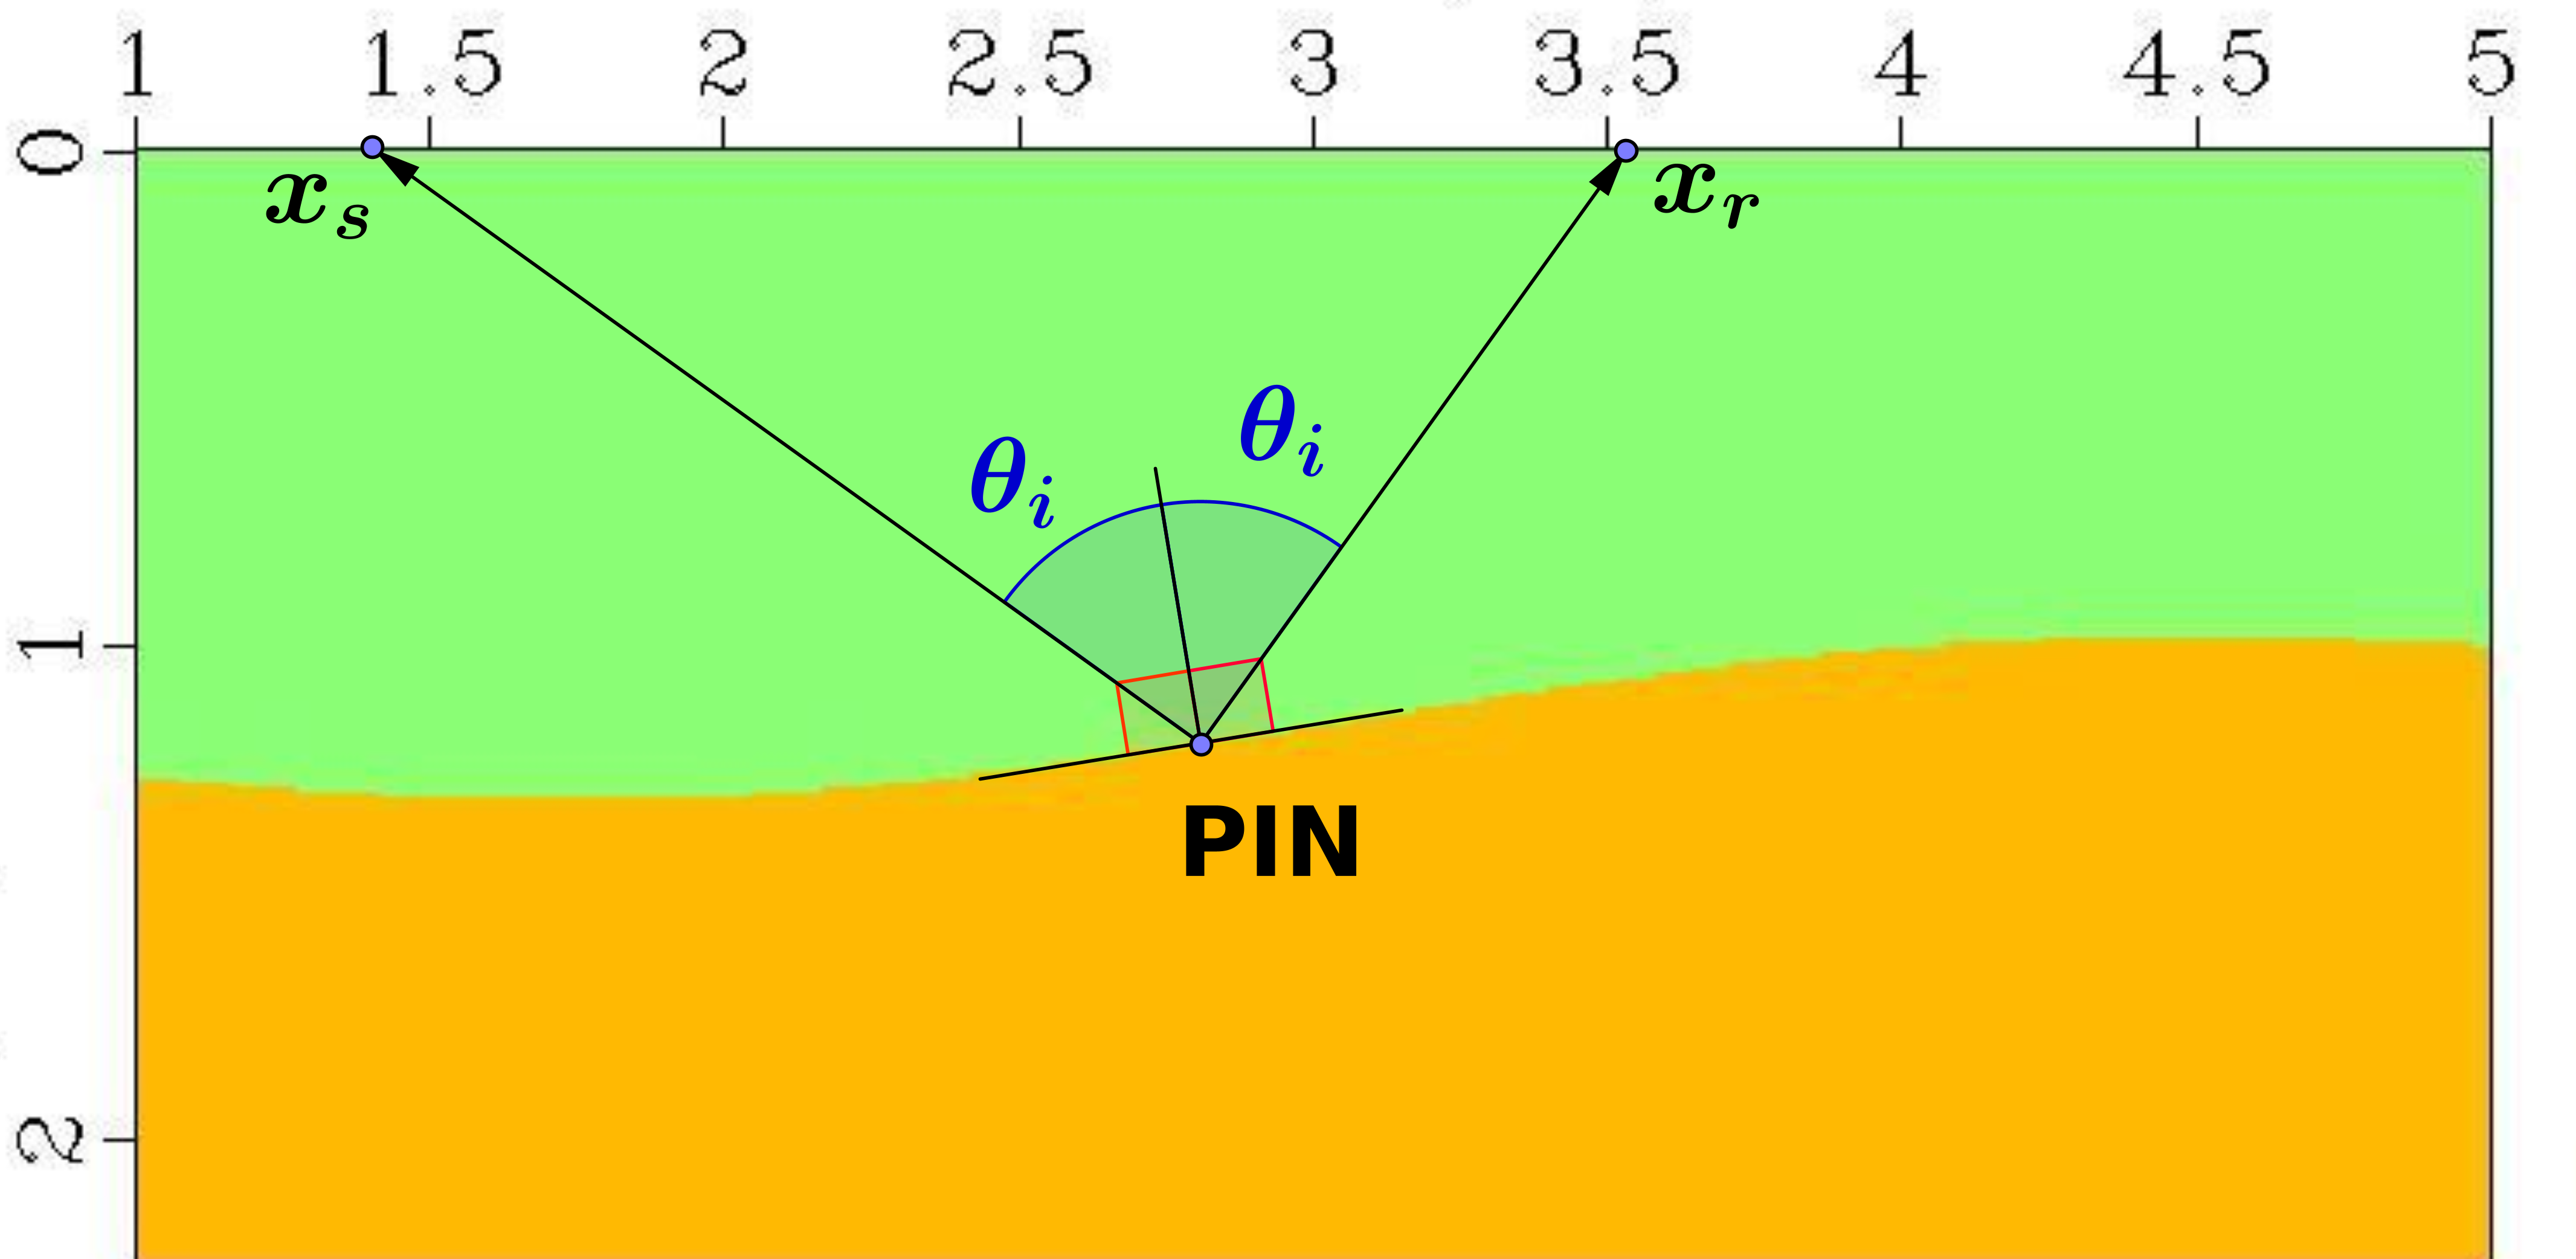
\includegraphics[scale=0.5]{images/modelagem2.png}
\vspace{-0.3cm}
\end{center}
\begin{center}
 Fonte: Do Autor.
\end{center}
\label{fig:9.8}
\end{figure}

Após a determinação da localização das fontes no modelo,
a modelagem direta é realizada através do traçamento de pares de raios de reflexão
iniciando nas posições das fontes PIN determinadas para um modelo de velocidades
inicial,
simulando uma família ERC de raios de reflexão que atingem a superfície de aquisição
na posição da fonte $x_s$ e do receptor $x_r$ (Figura \ref{fig:9.8}).
Este leque de raios é lançado em direção à superfície de aquisição,
os tempos de trânsito dos raios de reflexão são armazenados \cite{stereo}.
Os tempos de trânsito dos raios de reflexão obtidos no traçamento de raios são comparados com os tempos
de trânsito da aproximação de tempo de trânsito ERC a seguir \cite{cre}:

\begin{multline}
\label{eq:9.1}
t(h,m)= \left( \tau_0-\frac{2R_{NIP}}{v_0} \right) 
+\frac{R_{NIP}}{v_0}\sqrt{1-2\alpha(m-m_0+h)+\frac{(m-m_0+h)^2}{R_{NIP}^2}} \\
+\frac{R_{NIP}}{v_0}\sqrt{1+2\alpha(m-m_0-h)+\frac{(m-m_0-h)^2}{R_{NIP}^2}}
\end{multline}


Onde $m$ é a coordenada do PMC, $h$ é a coordenada do afastamento entre fonte e receptor e
$\alpha$ é um parâmetro de assimetria dado em função de $R_{NIP}$ e $\beta_0$.
As diferenças $e_i$ entre os tempos de trânsito do traçamento de raios e dos tempos de trânsito
calculados são somadas segundo a fórmula \cite{stoffa}:

\begin{equation}
\label{eq:9.2}
L_2 = \left[ \sum_{i=1}^{ND} |e_i|^2 \right]^\frac{1}{2}
\end{equation}

As posições $x_s$ e $x_r$ são dadas pelo traçamento de raios armazenando as coordenadas de chegada
na superfície de aquisição dos raios de reflexão simulados na modelagem direta. Estas coordenadas podem
ser transformadas nas coordenadas do afastamento $h$ e PMC $m$ pelas Equações a seguir:

\begin{equation}
\label{eq:9.3}
h = (x_r-x_s)/2
\end{equation}

\begin{equation}
\label{eq:9.4}
m = (x_r+x_s)/2
\end{equation}

Como $\beta_0$, $R_{NIP}$ são parâmetros conhecidos para cada raio normal e obtidos do empilhamento
ERC e $v_0$ é a velocidade próximo da superfície de aquisição, também conhecida, podemos calcular o
tempo de trânsito esperado com a Equação \ref{eq:9.1} e comparar com o tempo de trânsito do raio de
reflexão simulado
dado pela soma dos tempos $\Delta \tau_s$ e $\Delta \tau_r$,
do raio que sai do ponto PIN e chega em $x_s$
e do raio
que sai do ponto PIN e chega em $x_r$, respectivamente.
Esta diferença deve ser mínima para o modelo de velocidades
correto. A soma dos tempos de trânsito obtidas com o
traçamento de raios é dada a seguir:

\begin{equation}
\label{eq:9.5}
\tau(h,m) = \Delta \tau_s + \Delta \tau_r
\end{equation}

Assim, a diferença $e_i$ e a norma dois $L_2$ da Equação \ref{eq:9.2} podem ser estabelecidas como:

\begin{equation}
\label{eq:9.6}
L_2 = \left[ \sum_{i=1}^{ND} |e_i|^2 \right]^\frac{1}{2}
= \left[ \sum_{i=1}^{ND} |\tau(h,m)-t(h,m)|^2 \right]^\frac{1}{2}
\end{equation}

A norma dois das diferenças nos tempos de trânsito (Equação \ref{eq:9.2})
será utilizada como critério de
convergência do modelo de velocidades: O modelo de velocidades otimizado deverá produzir
o valor mínimo das diferenças entre os tempos de trânsito obtidos com o traçamento de raios
e calculados com a fórmula do ERC (Equação \ref{eq:9.1}). Assim, a estratégia de inversão consiste em
atualizar o modelo de velocidades utilizado de modo a
encontrar o modelo que produz o mínimo global da Equação \ref{eq:9.2}. O algoritmo de inversão
do modelo de velocidades é apresentado na Figura \ref{fig:9.9}.

A metodologia para a atualização do modelo de velocidades durante a inversão é utilizar o
Very Fast Simulated Annealing (VFSA) para atualizar parâmetros que definem o modelo de velocidades
em profundidade tomando como critério de convergência o valor calculado para a norma dois na Equação
\ref{eq:9.2}. Os parâmetros irão depender do modo de representação do modelo de velocidades, exemplo:
um modelo de velocidades em que a velocidade cresce linearmente com a profundidade depende do gradiente
de velocidades $g_z$ e da velocidade próximo da superfície de aquisição $v_0$. Considerando $v_0$ conhecida,
a atualização do modelo será dada pela atualização do gradiente $g_z$ como parâmetro otimizado pelo VFSA.

Esta estratégia de otimização é realizada em looping (Figura \ref{fig:9.10}),
utilizando o modelo de velocidades otimizado, resultado
da otimização anterior, como novo modelo de velocidades inicial. Assim, a localização das fontes PIN é
atualizada no início do processo de inversão para cada novo modelo de velocidades inicial utilizado.
Também ocorre a atualização do vetor vagarosidade na localização da fonte PIN e consequentemente
dos ângulos de chegada do raio normal nestes pontos.

\begin{figure}[H]
\caption{Representação esquemática do algoritmo de inversão do modelo de velocidades
a partir da estratégia apresentada neste capítulo.}
\begin{center}
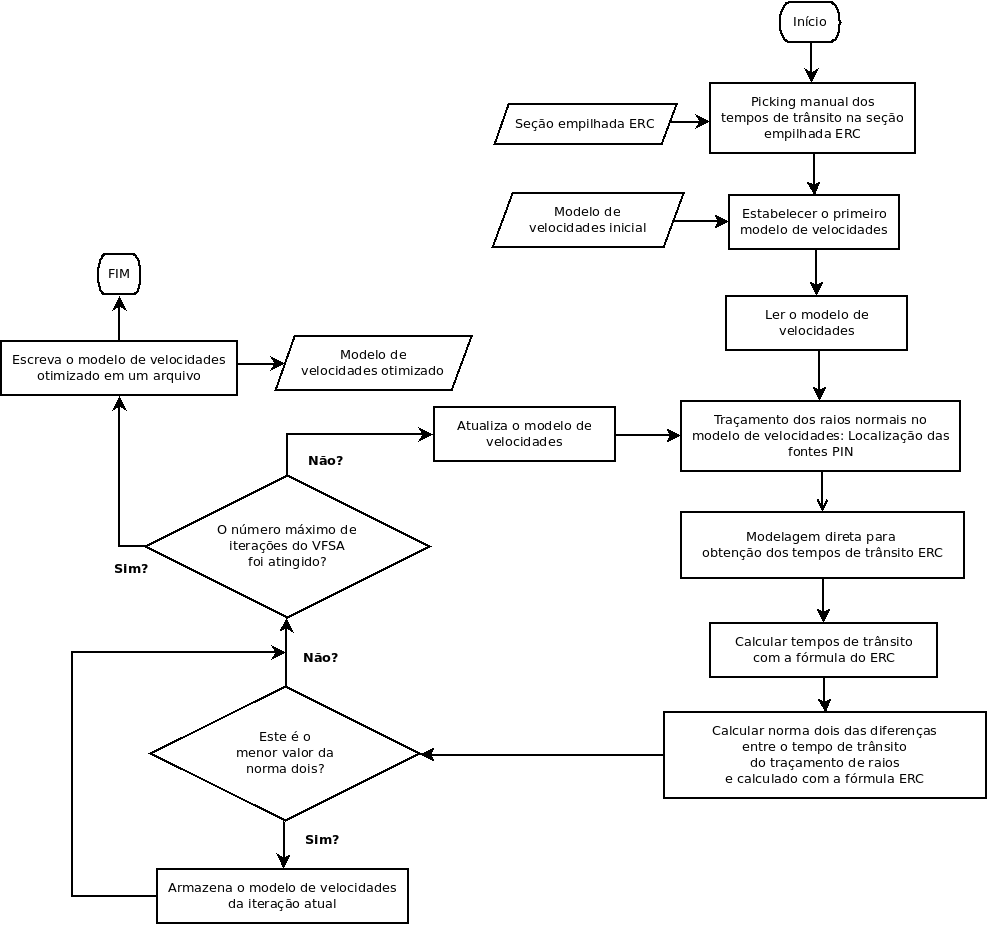
\includegraphics[scale=0.45]{images/fluxocomp.png}
\vspace{-0.3cm}
\end{center}
\begin{center}
 Fonte: Do Autor.
\end{center}
\label{fig:9.9}
\end{figure}

\begin{figure}[H]
\caption{Representação esquemática do algoritmo de inversão do modelo de velocidades
sendo utilizado em looping. O modelo de velocidades otimizado da iteração anterior é utilizado
como novo modelo de velocidades inicial e inversão é refeita.}
\begin{center}
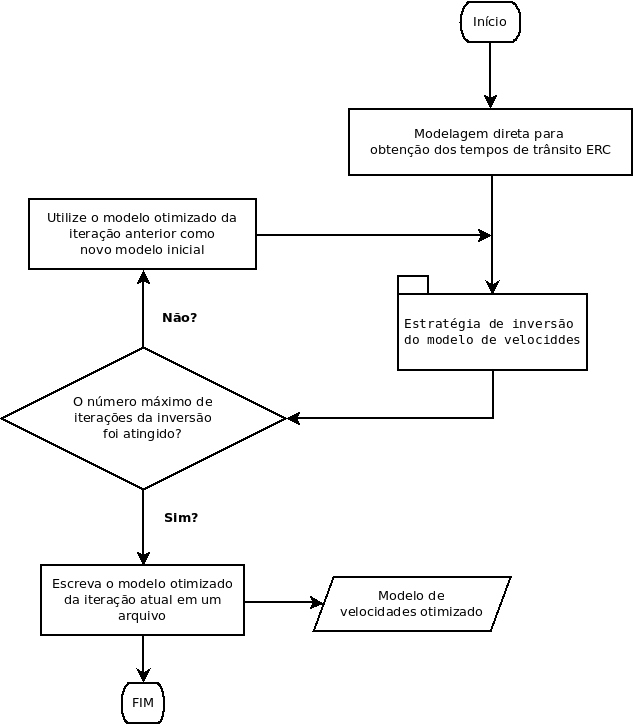
\includegraphics[scale=0.5]{images/fluxorepeat.png}
\vspace{-0.3cm}
\end{center}
\begin{center}
 Fonte: Do Autor.
\end{center}
\label{fig:9.10}
\end{figure}
